\documentclass[12pt]{article}
\usepackage{natbib}
\usepackage[french]{babel}
\usepackage[T1]{fontenc}
\usepackage{url}
\usepackage[utf8x]{inputenc}
\usepackage{amsmath}
\usepackage{mathtools}
\usepackage{graphicx}
\graphicspath{{images/}}
\usepackage{parskip}
\usepackage{amssymb}
\usepackage{xurl}
\usepackage{caption}
\usepackage{geometry}
\usepackage[shortlabels]{enumitem}
\geometry{hmargin = 2.5cm, vmargin = 2.5cm}

\title{}							% Title
\date{\today}											% Date

\makeatletter
\let\thetitle\@title
\let\theauthor\@author
\let\thedate\@date
\makeatother

\begin{document}
%%%%%%%%%%%%%%%%%%%%%%%%%%%%%%%%%%%%%%%%%%%%%%%%%%%%%%%%%%%%%%%%%%%%%%%%%%%%%%%%%%%%%%%%%

\begin{titlepage}
	\centering
    
\includegraphics[scale = 0.7]{img/University.png}\\[1.0 cm]	% University Logo
    \textsc{\LARGE \newline\newline Faculté des Sciences appliquées}\\	% University Name
	\textsc{\Large  ELEN062-1: Introduction to Machine Learning}\\[0.5 cm]	% Course Code
	\rule{\linewidth}{0.2 mm} \\[0.4 cm]
	{\huge \bfseries \thetitle}\\
	\rule{\linewidth}{0.2 mm} \\[2 cm]
	
	\begin{minipage}{0.5\textwidth}
		\begin{flushleft} \large
			\emph{Professeur:}\\
			Louis Wehenkel and Pierre Geurts\\
			\end{flushleft}
			\end{minipage}~
			\begin{minipage}{0.4\textwidth}
            
			\begin{flushright} \large
			\emph{Groupe:} \\
			LAMBERMONT Romain\\
            LOUIS Arthur\\
		\end{flushright}
        
	\end{minipage}\\[5 cm]
	
	
    \thedate
	
\end{titlepage}

%%%%%%%%%%%%%%%%%%%%%%%%%%%%%%%%%%%%%%%%%%%%%%%%%%%%%%%%%%%%%%%%%%%%%%%%%%%%%%%%%%%%%%%%%
\thispagestyle{empty}
\pagebreak
%%%%%%%%%%%%%%%%%%%%%%%%%%%%%%%%%%%%%%%%%%%%%%%%%%%%%%%%%%%%%%%%%%%%%%%%%%%%%%%%%%%%%%%%%
\setcounter{page}{1}
\section{Introduction}
\section{Classical algorithms}
\subsection{Decision trees}
\begin{enumerate}[a)]
	\item text
\begin{figure}[htp]
	\centering
	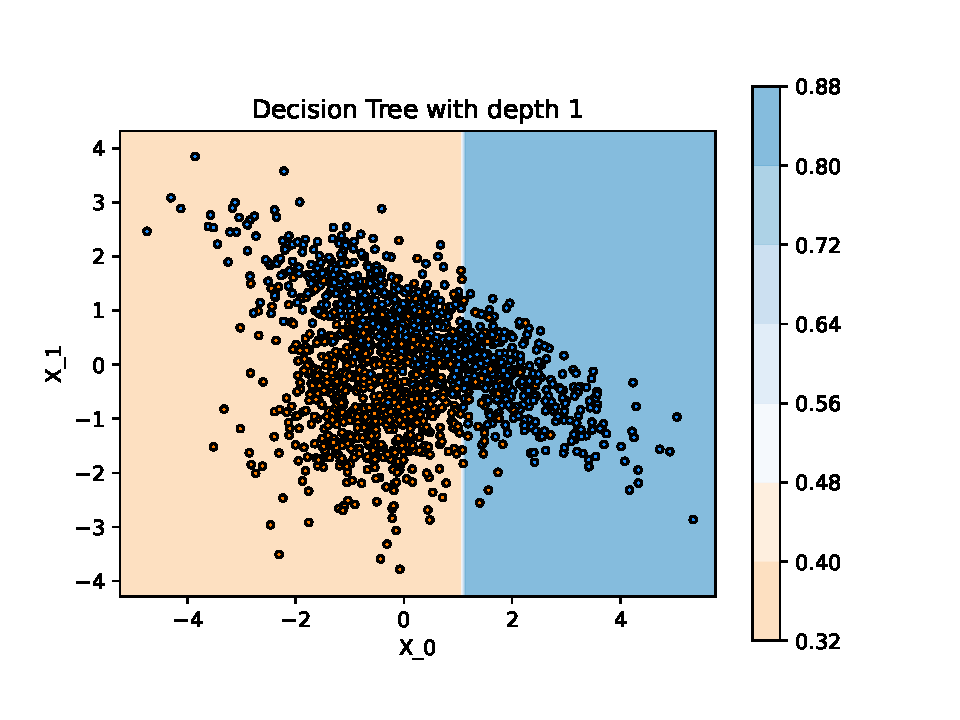
\includegraphics[width=.3\textwidth]{img/dt_1.pdf}\quad
	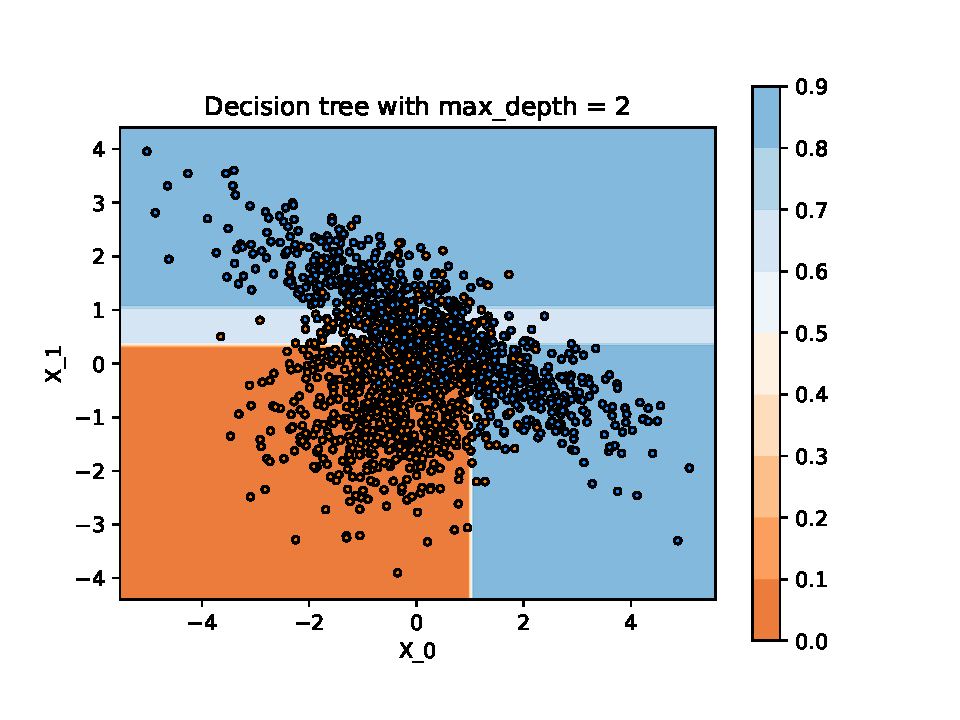
\includegraphics[width=.3\textwidth]{img/dt_2.pdf}\quad
	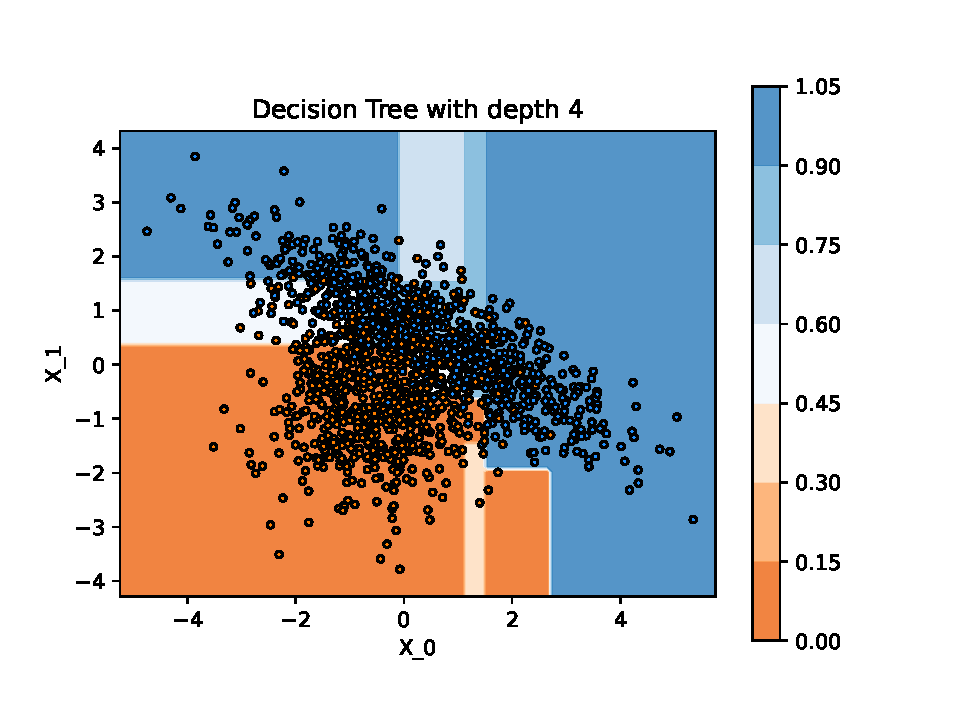
\includegraphics[width=.3\textwidth]{img/dt_4.pdf}
	
	\medskip
	
	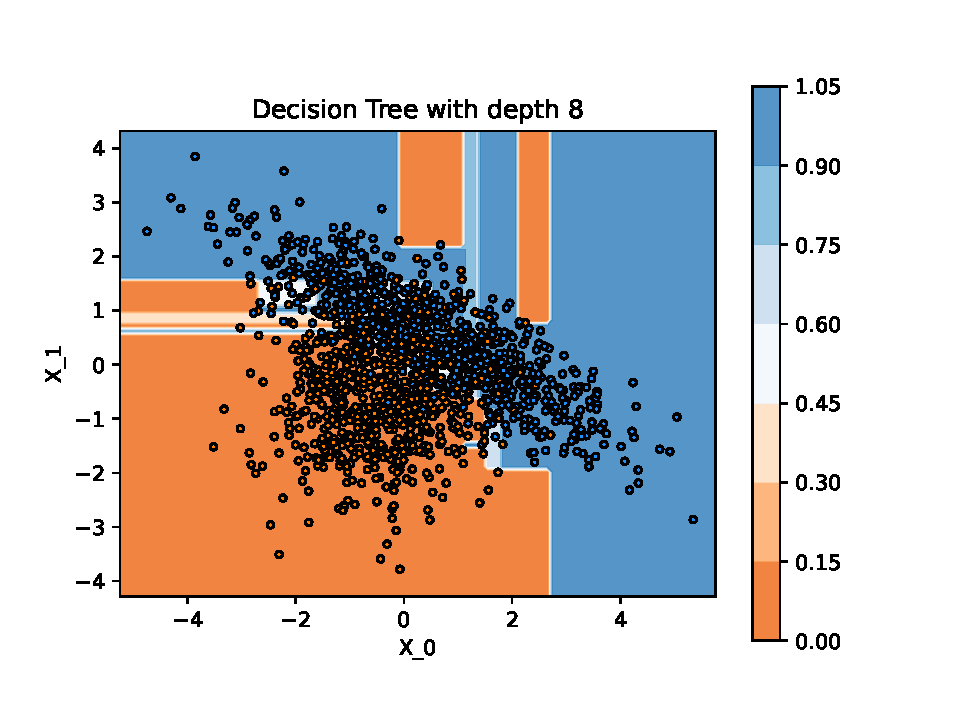
\includegraphics[width=.3\textwidth]{img/dt_8.pdf}\quad
	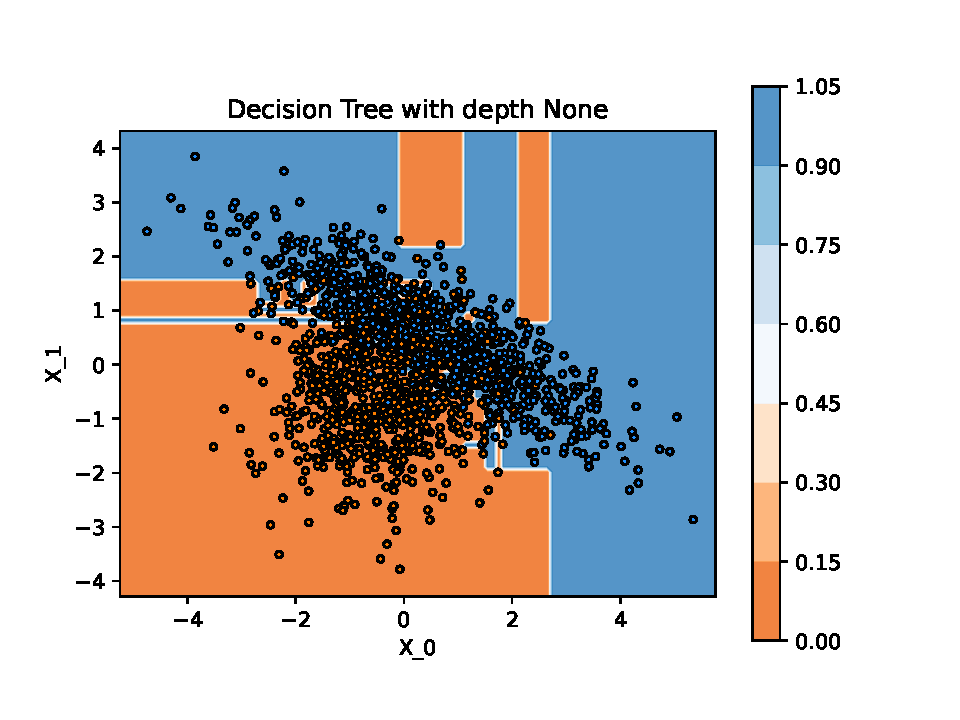
\includegraphics[width=.3\textwidth]{img/dt_None.pdf}
	
	\caption{Decision trees with different depths}
	\end{figure}
As we can see on the figure below the division of the 2 areas become more complex with the depths of the tree. The tree with a depth of 8 is overfitting the data. The tree with a depth of 1 is underfitting the data.
The depth 2 and 4 are the best compromise between underfitting and overfitting.
\end{enumerate}
\subsection{K-nearest neighbors}
\subsection{Quadratic/Linear discriminant analysis}
\section{Comparison}

\end{document} 